\section{Task 1}
Given a function $$y = \frac{\cos(x)}{x^3} - x^2$$ we want to calculate total
error introduced by inaccurate representation of $x$.
\subsection{Epsilon calculus}
To calculate error of representation, everywhere where there is an $x$, we need
to introduce $\epsilon$ as the error like so: $\tilde{x} = x(1+\epsilon)$
In our function we have:
\begin{align*}
    v_1 &= \cos(x) \\ 
    v_2 &= x^3 \\ 
    v_3 &= \frac{v_1}{v_2} \\ 
    v_4 &= x^2 \\ 
    y &= v_3 - v_4
\end{align*}
Therefore we obtain:
\begin{align*}
    \tilde{v_1} &= \cos(x(1+\epsilon_1)) \\ 
    \tilde{v_2} &= (x(1+\epsilon))^3 = x^3 (1+3\epsilon_2) \\ 
    \tilde{v_3} &= \frac{\tilde{v_1}}{\tilde{v_2}} \\ 
    \tilde{v_4} &= (x(1+\epsilon))^2 = x^2 (1+2\epsilon_3) \\
    \tilde{y} &= \tilde{v_3} - \tilde{v_4}
\end{align*}
Let us focus on $\tilde{ v_1 }$:
$$ \cos(x(1+\epsilon)) = \cos(x+x\epsilon) = \cos(x)\cos(x\epsilon) -
\sin(x)\sin(x\epsilon) $$
We need to use properties of trigonometric functions in order to solve it.
Those properties are listed in the section \textit{Mathematical Symbols and
formulas used}, formula (2). \\
Using those properties:
\begin{align*}
    \cos(x(1+\epsilon)) &= \cos(x)\cos(x\epsilon) - \sin(x)\sin(x\epsilon)\\
    &= \cos(x)(1-\frac{(x\epsilon)^2}{2}) - \sin(x)(x-\frac{(x\epsilon)^3}{6})\epsilon \\
    &= \cos(x) - \sin(x)x\epsilon\\
    &= \cos(x)\cdot (1-\tan(x)x\epsilon)
\end{align*}
Now solve $v_3$:
\begin{align*}
    \tilde{v_3} &= \displaystyle\frac{\cos(x) \cdot (1 - x\tan(x)
    \epsilon_1)}{x^3 (1+3\epsilon_2)}\\
    &= \frac{\cos(x)}{x^3} (1 - x\tan(x) \epsilon_1)\cdot (1+3\epsilon_2)^{-1}\\
    &= \frac{\cos(x)}{x^3} (1 - x\tan(x) \epsilon_1)\cdot (1-3\epsilon_2)\\
    &= \frac{\cos(x)}{x^3} (1 - x\tan(x) \epsilon_1 - 3\epsilon_2)
\end{align*}
Substituting it to the equation:
\begin{align*}
\tilde{y}&=\frac{\cos(x)}{x^3}(1 - x\tan(x) \epsilon_1 - 3\epsilon_2)-x^2(1+2\epsilon_3)\\
    &=\frac{\cos(x)}{x^3}-\frac{\cos(x)}{x^3}(x\tan(x) \epsilon_1 +
    3\epsilon_2)-x^2-2x^2\epsilon_3 \\
    &=y-\frac{\cos(x)}{x^3}(x\tan(x) \epsilon_1 + 3\epsilon_2)-2x^2\epsilon_3\\
    &=y(1 + (-\frac{\cos(x)}{x^3}(x\tan(x) \epsilon_1 +
    3\epsilon_2)-2x^2\epsilon_3)\frac1y)\\
    &=y\left(1 + \left(-\frac{\sin(x)}{x^2}\epsilon_1
    -3\frac{\cos(x)}{x^3}\epsilon_2 - 2x^2\epsilon_3\right)\frac1y\right)
\end{align*}
Therefore, using the formula (4):
$$T(x) = \displaystyle\frac{ \left|-\frac{\sin(x)}{x^2}\right| +
\left|- 3\frac{\cos(x)}{x^3}\right| + \left|-2x^2\right| }
{\frac{\cos(x)}{x^3} - x^2}$$

\subsection{Numerical simulation}
Function that we need to implement, described in an assignment:
$$T(x) = \frac{1}{\epsilon_{sim}}\left| \displaystyle\frac{y(\tilde{x}) - y(x)}{y(x)} \right|$$
is more general solution for calculating the error. It can be easily implemented 
in MATLAB code:
\begin{lstlisting}[language=MATLAB]
    y = @(x) cos(x)./x.^3 - x.^2;
    x_eps = x.*(1+esim);
    yeps = y(x_eps);
\end{lstlisting}
where anonymous function y can be reused for calculating "true" value of the function.

\subsection{Comparison of results}
Both methods do not differ significantly from one another in terms of results.
This can be seen on \ref{fig:task1}, where the output difference is barely
noticable. Therefore, the use of simpler solution should be recommended.
\begin{figure}[ht]
    \begin{center}
        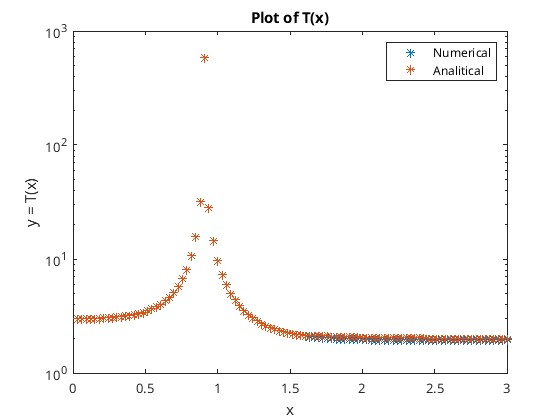
\includegraphics[width=\textwidth]{Task1.jpg}
    \end{center}
    \caption{Comparison of calculating error via numerical and analytical way}
    \label{fig:task1}
\end{figure}
